\documentclass[a4paper, 14pt]{extarticle}
\usepackage[utf8]{inputenc}
\usepackage[paper=a4paper, top=1cm, right=1cm, bottom=1.5cm, left=2cm]{geometry}
\usepackage{setspace}
\usepackage[russian]{babel}
\usepackage[T2A]{fontenc}
\usepackage{indentfirst}
\usepackage{pscyr}
\onehalfspacing

\usepackage{graphicx}

\parindent=1.25cm

\usepackage{titlesec}

\usepackage{caption}
\captionsetup{labelsep=period}


\titleformat{\section}
    {\normalsize\bfseries}
    {\thesection}
    {1em}{}

\titleformat{\subsection}
    {\normalsize\bfseries}
    {\thesubsection}
    {1em}{}

% Настройка вертикальных и горизонтальных отступов
\titlespacing*{\chapter}{0pt}{-30pt}{8pt}
\titlespacing*{\section}{\parindent}{*4}{*4}
\titlespacing*{\subsection}{\parindent}{*4}{*4}

\usepackage[square, numbers, sort&compress]{natbib}
\makeatletter
\bibliographystyle{unsrt}
\renewcommand{\@biblabel}[1]{#1.} 
\renewcommand{\theenumi}{\arabic{enumi}}
\renewcommand{\labelenumi}{\arabic{enumi}.}
\renewcommand{\theenumii}{.\arabic{enumii}}
\renewcommand{\labelenumii}{\arabic{enumi}.\arabic{enumii}.}
\renewcommand{\theenumiii}{.\arabic{enumiii}}
\renewcommand{\labelenumiii}{\arabic{enumi}.\arabic{enumii}.\arabic{enumiii}.}
\renewcommand{\baselinestretch}{1.5}
\makeatother


\newcommand{\maketitlepage}[6]{
    \begin{titlepage}
        \singlespacing
        \newpage
        \begin{center}
            Министерство образования и науки Российской Федерации \\
            Федеральное государственное бюджетное образовательное \\
            учреждение высшего профессионального образования \\
            <<Волгоградский государственный технический университет>> \\
            #1 \\
            Кафедра #2
        \end{center}


        \vspace{14em}

        \begin{center}
            \large Реферат по дисциплине
            \\ #3
        \end{center}

        \vspace{5em}

        \begin{flushright}
            \begin{minipage}{.3\textwidth}
                Выполнил:\\#4
                \vspace{1em}\\
                Проверил:\\#5
                \\
                \\ Оценка \underline{\ \ \ \ \ \ \ \ \ \ \ \ \ \ \ \ }
            \end{minipage}
        \end{flushright}

        \vspace{\fill}

        \begin{center}
            Волгоград, 2013
        \end{center}

    \end{titlepage}
    \setcounter{page}{2}
}

\begin{document}
\maketitlepage{Факультет электроники и вычислительной техники}
{<<Электронно-вычислительные машины и системы>>}
{Микроэлектроника и схемотехника \\ <<Типы памяти>>}
{студент группы Ф-369\\Голубев~А.~В.}{Черных~Д.~А.}{}

На текущий веток развития технологий нас окружают многочисленный технические 
изобретения, которые ещё вчера являлись чем-то фантастичным и невозможным. 
Прогресс не стоит на месте, с каждым днём в мире появляются новые интересные 
изобретения, от обычных безделушек до вычислительных кластеров. Наверное 
невозможно представить работу того либо другого устройства без жёстких 
дисков и модулей памяти. В текущем работе кратко рассмотрим некоторые 
типы памяти. \\

\emph{Память на магнитных сердечниках} (magnetic core memory) или ферритовая 
память (ferrite memory) -- запоминающее устройство, хранящее информацию 
в виде направления намагниченности небольших ферритовых сердечников, 
обычно имеющих форму кольца. Ферритовые кольца расставлялись в 
прямоугольную матрицу и через каждое кольцо проходило (в зависимости от 
конструкции запоминающего устройства) от двух до четырёх проводов для 
считывания и записи информации. Память на магнитных сердечниках была 
основным типом компьютерной памяти с середины 1950-х и до середины 
1970-х годов.

\begin{wrapfigure}[11]{l}{0.5\textwidth}
    \vspace{-2ex}
    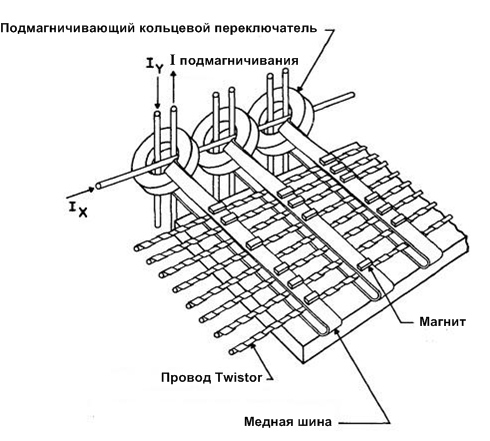
\includegraphics[width=0.5\textwidth]{images/image_01}
    \parbox{0.5\textwidth}{\caption{Схематическое представление}}
\end{wrapfigure}

В это время существовало несколько вариантов памяти на магнитных 
сердечниках, но наиболее существенный тип, который подтолкнул 
дальнейшее развитие это: твистор-память (twistor memory)

Суть твистор-памяти: массив пермаллоевых псевдоколец продетых через 
один несущий провод. Кольца же были образованы свёрнутым зигзагообразным 
проводом на который навивалась фольга из пермаллоя под углом в сорок пять
градусов.

\hspace{-6ex}\begin{minipage}[h]{0.5\linewidth}
\vspace{5ex}Плюсы:
\begin{enumerate}[noitemsep]
	\item возможность чтения или записи целой строки пермаллоевых псевдоколец 
	\item компактность
\end{enumerate}
\end{minipage}
\begin{minipage}[h]{0.5\linewidth}
Минусы:
\begin{enumerate}[noitemsep]
	\item проигрыш памяти DRAM в энергопотреблении
\end{enumerate}
\end{minipage} \\\\

\emph{Сегнетоэлектрическая оперативная память} (Ferroelectric RAM, FeRAM или 
FRAM) -- оперативная память, по своему устройству схожая с DRAM, но 
использующая слой сегнетоэлектрика вместо диэлектрического слоя для 
обеспечения энергонезависимости. FeRAM -- одна из растущего числа 
альтернативных технологий энергонезависимой памяти, предлагающая ту же 
самую функциональность, что и флеш-память.

\begin{wrapfigure}[11]{l}{0.5\textwidth}
    \vspace{-2ex}
    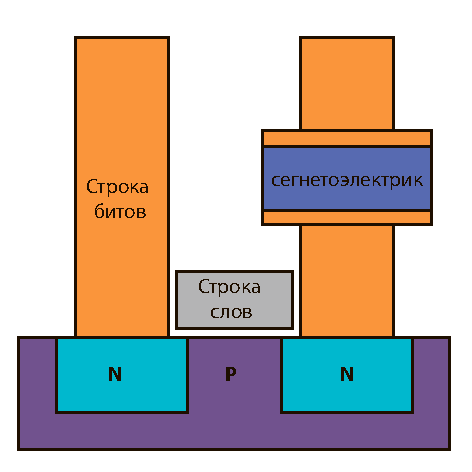
\includegraphics[width=0.5\textwidth]{images/image_02}
    \parbox{0.5\textwidth}{\caption{Структура ячейки памяти}}
\end{wrapfigure}

Функционально FeRAM схожа с DRAM, только для хранения информации 
используют сегнетоэлектрик и запись происходит путем проникновения 
поля через сегнетоэлектрический слой при заряжании электродов,
принуждая атомы внутри принимать ориентацию вверх или вниз 
(в зависимости от полярности заряда), за счет чего запоминается 
<<1>> или <<0>>. \\

\hspace{-5ex}\begin{minipage}[h]{0.5\linewidth}
\vspace{2ex}Плюсы:
\begin{enumerate}[noitemsep]
	\item низкое энергопотреблении
	\item быстрая скорость записи
	\item большое число циклов перезаписи
\end{enumerate}
\end{minipage}
\begin{minipage}[h]{0.5\linewidth}
Минусы:
\begin{enumerate}[noitemsep]
	\item низкая плотность информации 
	\item ограниченная ёмкость
	\item высокая стоимость
\end{enumerate}
\end{minipage}

\pagebreak

\emph{Магниторезистивная память} (MRAM) -- одно из перспективных направлений 
новых типов памяти. В ближайшем будущем она может превзойти все 
существующие виды памяти по всем характеристикам. Ячейки MRAM сравнимы по 
быстродействию с SRAM -- памятью, которая используется в кэше процессора, 
по плотности ячеек -- c DRAM. Память MRAM энергонезависима и она гораздо 
экономичнее и долговечнее флэш-памяти.

\begin{wrapfigure}[11]{l}{0.5\textwidth}
   \vspace{-2ex}
    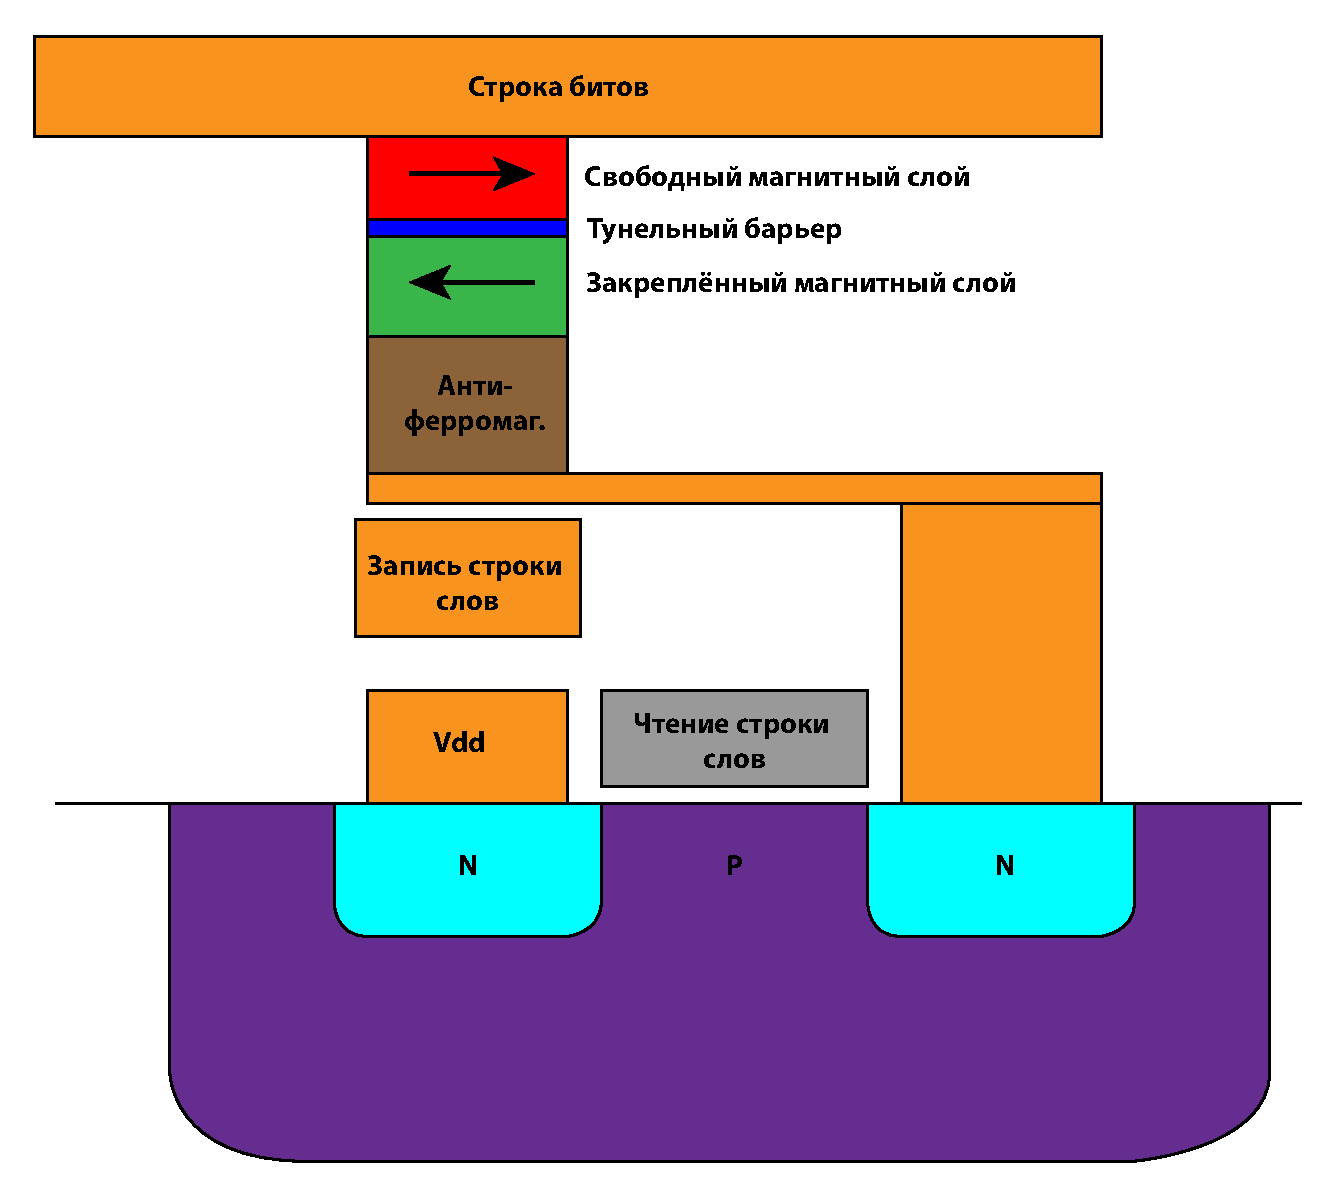
\includegraphics[width=0.5\textwidth]{images/image_03}
    \parbox{0.5\textwidth}{\caption{Структура}}
\end{wrapfigure}

Информация в ячейках MRAM хранится в двух ферромагнитных слоях, 
разделённых тонким слоем диэлектрика. Один из слоёв -- постоянный магнит, 
направление магнитного поля второго слоя может меняться. Для изменения 
магнитного поля через ячейку пропускают ток. От взаимной ориентации полей в 
этих слоях зависит электрическое сопротивление ячейки. Измеряя это 
сопротивление, можно считать хранящийся в ячейке бит. На сегодня самый 
совершенный способ записи используют эффект переноса спинового момента -- 
<<поляризованные>> электроны, проходя через слой ферромагнетика, помогают 
вращать магнитное поле в определённом направлении, в результате чего 
требуется гораздо меньший ток, и ячейки могут быть меньшего размера.

Исследователи Калифорнийского университете в Лос-Анджелесе (UCLA) нашли 
способ переключать магнитное поле с помощью электрического напряжения, а 
не тока, благодаря чему можно получить выигрыш в энергопотреблении от 
10 до 1000 раз, соответственно уменьшить нагрев ячеек в процессе записи 
и увеличить плотность их размещения на кристалле в 5 раз. Они называют 
это вид памяти MeRAM (magnetoelectrix random access memory).

\pagebreak

\emph{Phase-change memory} (память на основе фазового перехода) 
(также известна как PCM, PRAM, PCRAM, Ovonic Unified Memory, 
Chalcogenide RAM и C-RAM) -- новый тип энергонезависимой памяти. 
PRAM основывается на уникальном поведении халькогенида, который при 
нагреве может <<переключаться>> между двумя состояниями: кристаллическим 
и аморфным. 

\begin{wrapfigure}[9]{l}{0.5\textwidth}
    \vspace{-2ex}
    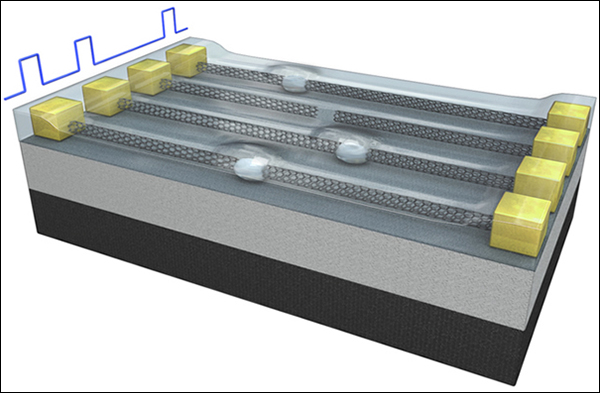
\includegraphics[width=0.5\textwidth]{images/image_04}
    \parbox{0.5\textwidth}{\caption{Схематическое представление}}
\end{wrapfigure}

В последних версиях смогли добавить ещё два дополнительных 
состояния, эффективно удвоив информационную емкость чипов. PRAM -- одна из
новых технологий памяти, созданная в попытке превзойти в области 
энергонезависимой памяти почти универсальную флеш-память, обладающую некоторым 
количеством практических проблем, решить которые как раз надеялись в PRAM.

\hspace{-5ex}\begin{minipage}[h]{0.5\linewidth}
\vspace{4ex}Плюсы:
\begin{enumerate}[noitemsep]
	\item быстрое переключение
	\item большое число циклов перезаписи
	\item устойчивость к радиации
\end{enumerate}
\end{minipage}
\begin{minipage}[h]{0.5\linewidth}
Минусы:
\begin{enumerate}[noitemsep]
	\item чувствительность к температуре
	\item высокая стоимость
\end{enumerate}
\end{minipage}

\pagebreak

Список литературы:
\vspace{-2ex}\begin{enumerate}[noitemsep]
	\item http://old.computerra.ru/vision/621983/
	\item http://old.computerra.ru/vision/622225/
	\item http://www.habrahabr.ru/post/163749
    \item http://ru.wikipedia.org/wiki/Память\_с\_изменением\_фазового\_состояния
\end{enumerate} 

\end{document}
